\documentclass[tikz,border=10pt]{standalone}
\begin{document}
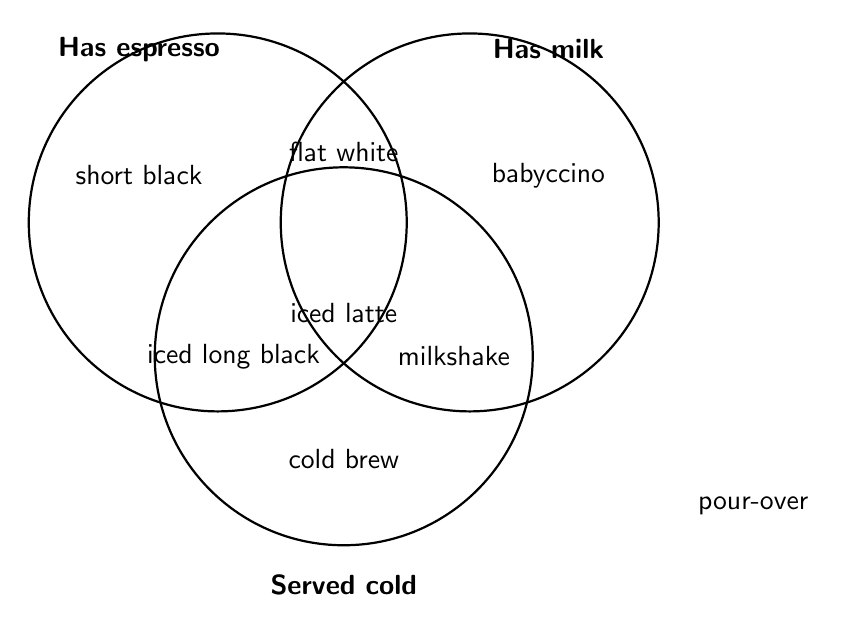
\begin{tikzpicture}[font=\sffamily]
  % three overlapping circles
  \draw[thick] (-1.6,0) circle (2.4);
  \draw[thick] (1.6,0) circle (2.4);
  \draw[thick] (0,-1.7) circle (2.4);

  % labels
  \node[font=\sffamily\bfseries] at (-2.6,2.2) {Has espresso};
  \node[font=\sffamily\bfseries] at (2.6,2.2) {Has milk};
  \node[font=\sffamily\bfseries] at (0,-4.6) {Served cold};

  % regions
  \node at (-2.6,0.6) {short black};      % espresso only
  \node at (2.6,0.6) {babyccino};         % milk only
  \node at (0,0.9) {flat white};          % espresso + milk
  \node at (-1.4,-1.7) {iced long black}; % espresso + cold
  \node at (1.4,-1.7) {milkshake};        % milk + cold
  \node at (0,-1.15) {iced latte};        % all three
  \node at (0,-3.0) {cold brew};          % cold only
  \node at (5.2,-3.6) {pour-over};        % outside all
\end{tikzpicture}
\end{document}
